%% If you have any problems using this template, please contact the author: %%
%% timhosgood@gmail.com. Updated for Statistics by SRH. Contact %%
%% ithelp@stats.ox.ac.uk if you have questions. %%
\documentclass{beamer}
\usepackage[utf8]{inputenc}
\usepackage{charter}
\usepackage{tikz}
\usepackage{graphicx}
\usepackage{amsmath}
\usepackage{mathtools}
\usepackage{amssymb}
\usepackage{pgfpages}
\usepackage[natbib=true,style=authoryear,backend=bibtex,useprefix=true]{biblatex}
\setbeamercolor*{bibliography entry title}{fg=black}
\setbeamercolor*{bibliography entry location}{fg=black}
\setbeamercolor*{bibliography entry note}{fg=black}
\setbeamertemplate{bibliography item}{}
\renewcommand*{\bibfont}{\scriptsize}
\addbibresource{bibliography_presentation.bib}

% \setbeameroption{show notes on second screen=right} % comment to get rid of notes
% \setbeamertemplate{note page}{\pagecolor{yellow!5}\insertnote}\usepackage{palatino}

% Defining custom macros
\renewcommand{\cal}[1]{\mathcal{#1}}
\newcommand{\scr}[1]{\mathscr{#1}}
\newcommand{\bb}[1]{\mathbb{#1}}

% Common sets
\newcommand{\R}{\mathbb{R}}
\newcommand{\N}{\mathbb{N}}
\newcommand{\Z}{\mathbb{Z}}

% Expectation
\newcommand{\E}{\mathbb{E}}
\newcommand{\Ex}[1]{\mathbb{E}\left[ #1 \right]}
\newcommand{\ExCond}[2]{\mathbb{E} \left[\left. #1 \right| #2 \right]}

% Probability
\renewcommand{\P}{\mathbb{P}}
\renewcommand{\Pr}[1]{\mathbb{P} \left( #1 \right)}
\newcommand{\PrCond}[2]{\mathbb{P} \left( \left. #1 \right| #2 \right)}

% Common distributions 
\newcommand{\dNorm}[2]{\mathcal(N)\left( #1, #2 \right)}
\newcommand{\dExp}[1]{\text{Exp} \left( #1 \right)}
\newcommand{\dBer}[1]{\text{Ber} \left( #1 \right)}
\newcommand{\dPoi}[1]{\text{Po} \left( #1 \right)}

% Miscellaneous math stuff
\newcommand{\defeq}{\vcentcolon=}
\newcommand{\eqdef}{=\vcentcolon}
\DeclarePairedDelimiter\ceil{\lceil}{\rceil}
\DeclarePairedDelimiter\floor{\lfloor}{\rfloor}
\newcommand{\powerset}{\raisebox{.15\baselineskip}{\Large\ensuremath{\wp}}}

\newtheorem{remark}{Remark}

%% Title slide formatting %%
\pgfdeclareimage[width=1.5cm]{statslogo}{images/Stats-logo.png}
\pgfdeclareimage[width=4cm]{lmslogo}{images/LMS_logo.png}
\pgfdeclareimage[width=3.3cm]{manifestation}{images/G_Mani.png}
\definecolor{oxfordblue}{RGB}{4,30,66}
\setbeamerfont{title}{size=\huge}
\setbeamerfont{author}{size=\normalsize}
\setbeamerfont{subtitle}{size=\small}
% Set the background colour to Oxford Blue
\setbeamercolor{background canvas}{bg=oxfordblue}

\setbeamertemplate{title page}{
    \begin{picture}(0,0)
        \put(-28.5,-163){%
			\pgfuseimage{manifestation}
        }
        \put(75,-105){%
            \begin{minipage}[b][4.5cm][t]{0.8\textwidth}
                \color{white}
                \usebeamerfont{title}
                    {\inserttitle\\[0.3cm]}
                     \usebeamerfont{subtitle}
                    {\insertsubtitle\\[0.5cm]}
                \usebeamerfont{author}               
                    {\insertauthor\\[0.3cm]}
                \tiny                                 
                    {\insertinstitute\\[0.3cm]}
                    {\insertdate}
            \end{minipage}        
        }
        \put(280,35){%
        	\pgfuseimage{statslogo}
        }
        \put(75,50){%
        	\pgfuseimage{lmslogo}
        }		
    \end{picture}
}

%% General slide formatting %%
\definecolor{oxfordblue}{RGB}{4,30,66}
\pgfdeclareimage[height=1cm]{statsbluelogo}{images/Stats-logo-RGB.png}

\setbeamertemplate{headline}
{%
    \begin{picture}(0,0)
        \put(320,-30){%
            \pgfuseimage{statsbluelogo}
        }
        \put(20,-35){%
             \rule{320pt}{0.4pt}
         }
    \end{picture}
}

\setbeamerfont{frametitle}{size=\Large}
\setbeamerfont{framesubtitle}{size=\normalsize}
\setbeamertemplate{frametitle}
{%

    \begin{picture}(0,0)
        \put(-8,-10){%
			\color{oxfordblue}
			\usebeamerfont{frametitle}{\insertframetitle}
        }
        \put(-7,-24){%
			\color{oxfordblue}
			\usebeamerfont{framesubtitle}{\insertframesubtitle}
        }            
    \end{picture}
}

\setbeamertemplate{footline}
{%
    \begin{picture}(0,0)
        \put(20,23){%
            \rule{320pt}{0.4pt}
        }
        \put(20,14){%
            \color{oxfordblue}\insertshortdate
        }
        \put(160,14){%
            \color{oxfordblue}\insertshorttitle
        }
        \put(337,14){%
            \color{oxfordblue}\insertframenumber
        }
    \end{picture}%
}
% Date customisation
\renewcommand{\today}{\number\day\space \ifcase\month\or
  January\or February\or March\or April\or May\or June\or
  July\or August\or September\or October\or November\or December\fi
   \space\number\year}

%% Information (author, title, etc.) %%

\title[Patrik Gerber (patrik.gerber@ccc.ox.ac.uk)]{The oriented contact \\process and the \\East model}
 % short title for footer
\author%
{%
    Patrik Gerber supervised by Prof. Paul Chleboun \\[0.1cm]
    \tiny{Supported by LMS and the Mathematical Institute, University of Oxford. }
}
\institute%
{%
    Department of Statistics\\
    University of Oxford
}

\date{4 October 2018}

%% Content of slides %%
\begin{document}
    \begin{frame}[plain]
        \titlepage
    \end{frame}
% Return default slide background colour to white.
\setbeamercolor{background canvas}{bg=white}
%

\begin{frame}
\frametitle{Overview}
\tableofcontents
\note{
Let me first give you an overview of what my project was about. It started out primarily concerned with the East-process. The idea was to apply a recent comparison based method that yielded new results for a different process. The corresponding results for the East process are already known, but an alternative, shorter proof could give indication that this comparison method could be useful for other KCMs of oriented nature, the class of processes that the East process belongs to. Upon reviewing the literature it became apparent that the necessary results for the oriented contact process were never precisely stated or proven even though the machinery had been developed. In the past 6 weeks we created a self contained proof of the necessary results and apply them to prove a weaker version of the known mixing time results for the East process. 
}
\end{frame}

%----------------------------------------------------------------------------------------
%	PRESENTATION SLIDES
%----------------------------------------------------------------------------------------

\section{East process}
\begin{frame}
\frametitle{East process}
\pause
\begin{block}{}
\vspace{-2mm}
The East process is a continuous time Markov chain
\pause. 
\begin{itemize}
\vspace{-1mm}
\item State space: $\Omega \defeq \{0, 1\}^\mathbb{Z}$, or equivalently, $\powerset(\mathbb{Z})$. 
\pause
\vspace{-1mm}
\item Each site $x \in \mathbb{Z}$ updates with rate $1$ to $B \sim \text{Ber}(p),\,p\in(0,1)$ \alert{iff} $x - 1$ is occupied. 
\end{itemize}
\end{block}
\vspace{-5mm}
\pause
\begin{figure}[!h]
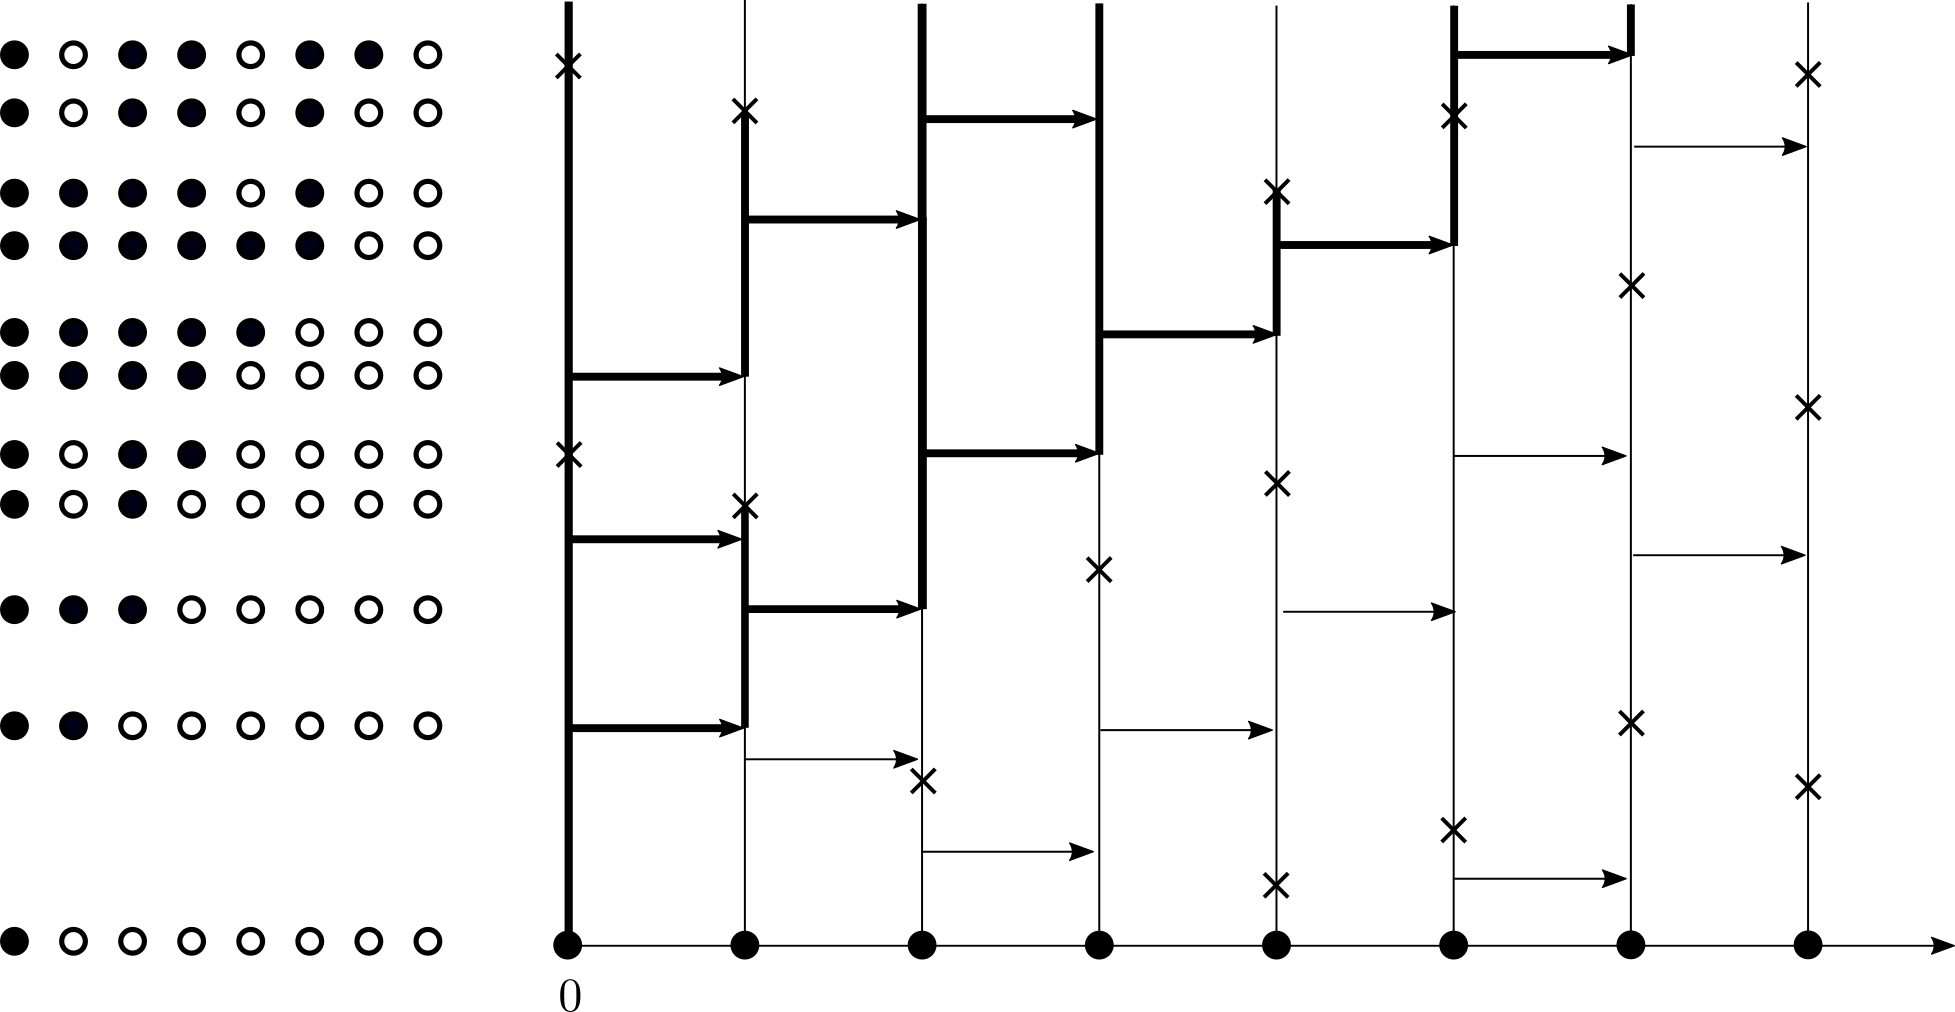
\includegraphics[scale=0.9]{images/East_graphical_construction}
\caption{East process started from $\{0\}$}
\end{figure}
\note{
\begin{enumerate}
\item So let me introduce the East process to you.
\item read slide 
\item Its state space is the set of configurations of 0s and 1s on the Integer lattice. Talk about powerset. 
\item Talk about graphical representation. Point out cross that doesn't kill spin. 
\end{enumerate}
}
\end{frame}

\section{Front propagation}
\begin{frame}
\frametitle{Front propagation}
\pause
\begin{definition}[Front]
Let $(\sigma_t)_{t \geq 0}$ be an East process started from $\{0\}$. The front of $(\sigma_t)_{t \geq 0}$  is the rightmost occupied site, written $X(\sigma_t) \defeq \sup\sigma_t$. 
\end{definition}
\pause
\begin{theorem}[{{\cite[Lemma 3.2]{blondel2013front}}}]
There exist constants $0 < \alpha < v$ and $\gamma, C > 0$ such that
\begin{align*}
\Pr{X(\sigma_t) \in (\alpha t, v t)} &\geq 1 - C e^{- \gamma t} &&\forall t \geq 0.
\end{align*}
\end{theorem}
\pause
\begin{proof}
We propose an alternative proof (under restrictions on $p$) detailed later. 
\end{proof}
\note{
\begin{enumerate}
\item The first step towards the proof of the linearity of the mixing time is a result about the front of the East process
\item Read slide 
\item Read theorem. What this says is ... .  
\item We give an alternative proof but for now, assuming this result, we can go on to show the desired linearity of the mixing time. 
\end{enumerate}
}
\end{frame}

\section{Mixing time}
\begin{frame}
\frametitle{Mixing time}
\pause
Restricted to $\{0, 1, ... L\}$ with a fixed 1 at origin East process converges to equilibrium. 
\pause
\begin{theorem}[{{\cite[Theorem 6.1]{cancrini2008kinetically}}}]
The mixing time of the East process on $\{0, 1, ... L\}$ with a fixed $1$ at the origin is $\Theta(L)$. 
\end{theorem}
\pause
\begin{proof}[Alternative proof using only front propagation]
Upper bound: Coupling time vs. propagation of the front. \\
Lower bound: Hitting times of large sets (\cite{peres2015mixing}). 
\end{proof}
\note{
\begin{enumerate}
\item I hope you are all familiar with the mixing time of a Markov chain. 
\item Talk about restriction to [0, L]
\item Read theorem.   
\item Talk about how to use front to prove this. Talk about restriction on $p$. 
\end{enumerate}
}
\end{frame}

\section{One-sided contact process}
\begin{frame}
\frametitle{One-sided contact process}
\pause
\begin{block}{}
The one-sided contact process is similar to the East process, but `recovery` is unconstrained. 
\end{block}
\pause
\begin{figure}[!h]
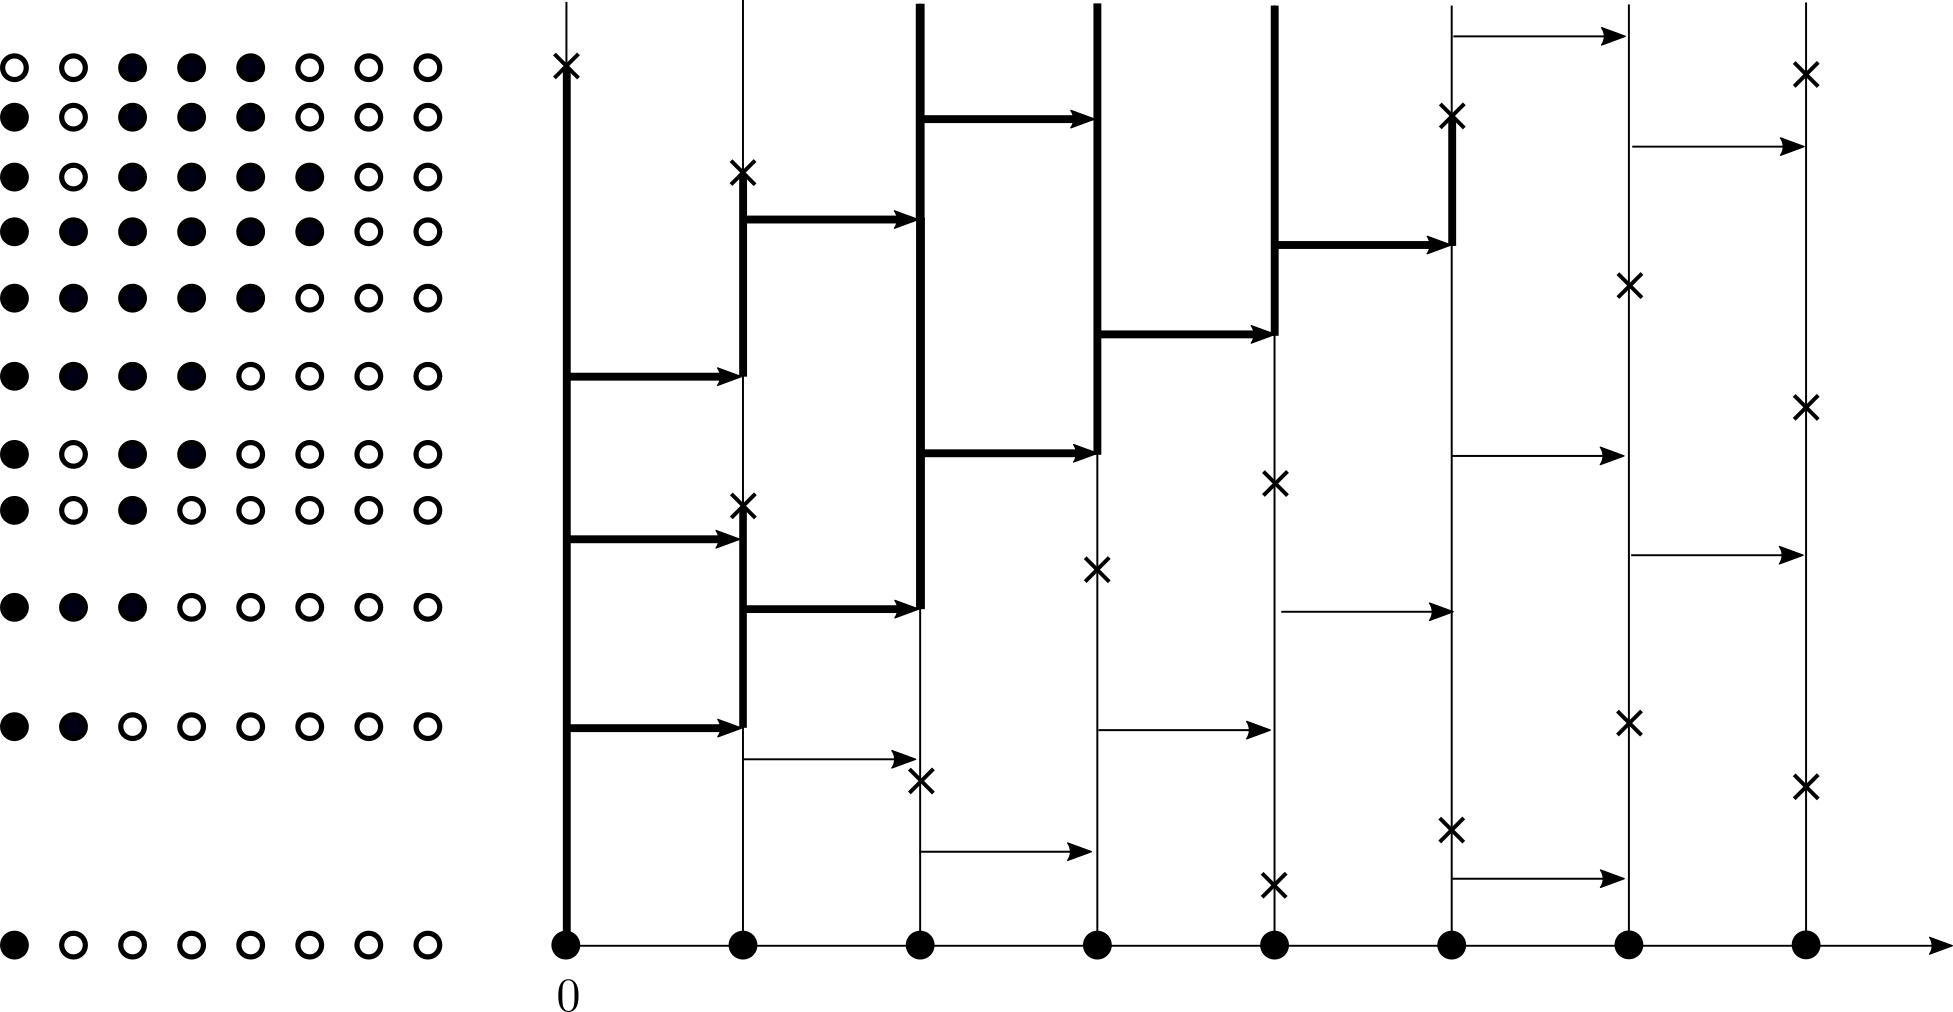
\includegraphics[scale=0.9]{images/graphical_construction}
\caption{One-sided contact process started from $\{0\}$}
\end{figure}
\note{
\begin{enumerate}
\item So I explained how the front propagation result can be used to prove the mixing time. But how do we prove the front propagation result? This is where the comparison technique comes in. Instead of studying the spectral gap of the East process, we compare it to a somewhat simpler process - the one-sided/oriented contact process. 
\item Explain how basic and oriented contact process works. 
\item Point out that cross always implies death. 
\end{enumerate}
}
\end{frame}

\section{East vs contact}
\begin{frame}
\frametitle{East vs Contact}
\pause
Same graphical structure for East and contact processes $\Rightarrow$ `basic coupling`. \\
\pause
Under the basic coupling
\begin{align*}
(\text{Oriented contact process}) \hspace{2mm} \eta_{t} &\leq \sigma_{t} \hspace{2mm} (\text{East process}) &&\forall t \geq 0. 
\end{align*}
\pause
In particular, 
\begin{align*}
X(\eta_{t}) &\leq X(\sigma_{t}) &&\forall t \geq 0. 
\end{align*}
\pause
For this to be useful, we need $p > p_c$ where $p_c \defeq \sup\{ p : |\eta| \rightarrow 0\ a.s.\}$. From here on consider only such $p$. 
\note{
\begin{enumerate}
\item How do we actually compare the two?
\item Basic coupling
\item Partial order and how its preserved
\item Front
\item Critical value and why its important
\end{enumerate}
}
\end{frame}

\section{Results for one-sided contact process}
\begin{frame}
\frametitle{Results for one-sided contact process}
\pause
\vspace{2mm}
Let $\tau(\eta_\cdot)$ be the extinction time. Then
\begin{align*}
\Pr{\tau(\eta_\cdot) = \infty} &> 0 &&\forall p > p_c. 
\end{align*} 
\pause
\vspace{-7mm}
\begin{theorem}
If $p > p_c$, there exists $\alpha > 0$ such that for all $a < \alpha$ there exist constants $\gamma, C > 0$ such that
\begin{align*}
  \PrCond{X(\eta_t) < a t}{\tau(\eta_\cdot) = \infty} &\leq C e^{-\gamma t} &&\forall t \geq 0. 
  \intertext{Furthermore there exist constants $\gamma, C > 0$ such that}
  \Pr{t < \tau(\eta_.) < \infty } &\leq C e^{-\gamma t} &&\forall t \geq 0.  
\end{align*}
\end{theorem}
\pause
\vspace{-5mm}
\begin{remark}
Hinted at in \cite{durrett1983supercritical} but never proved in detail. 
\end{remark}
\note{
\begin{enumerate}
\item There are some results that we need for the oriented contact process. 
\item Extinction time
\item Read theorem and explain
\item These results were never written down or proven in detail before.
\end{enumerate}
}
\end{frame}

\section{Percolation construction}
\begin{frame}
\frametitle{Percolation construction 1}
\pause
\vspace{1mm}
\begin{definition}
$\{(z(r), r)\}_{r \in [t,s]} \subset \Z \times \R_{\geq 0}$ is a \textit{path} if it follows arrows and goes through no cross. 
\end{definition}
\pause
\begin{figure}[!h]
\includegraphics[scale=0.85]{images/path}
\caption{Red and blue lines are examples of a path. }
\end{figure}
\end{frame}

\begin{frame}
\frametitle{Percolation construction 2}
\pause
\begin{figure}[!h]
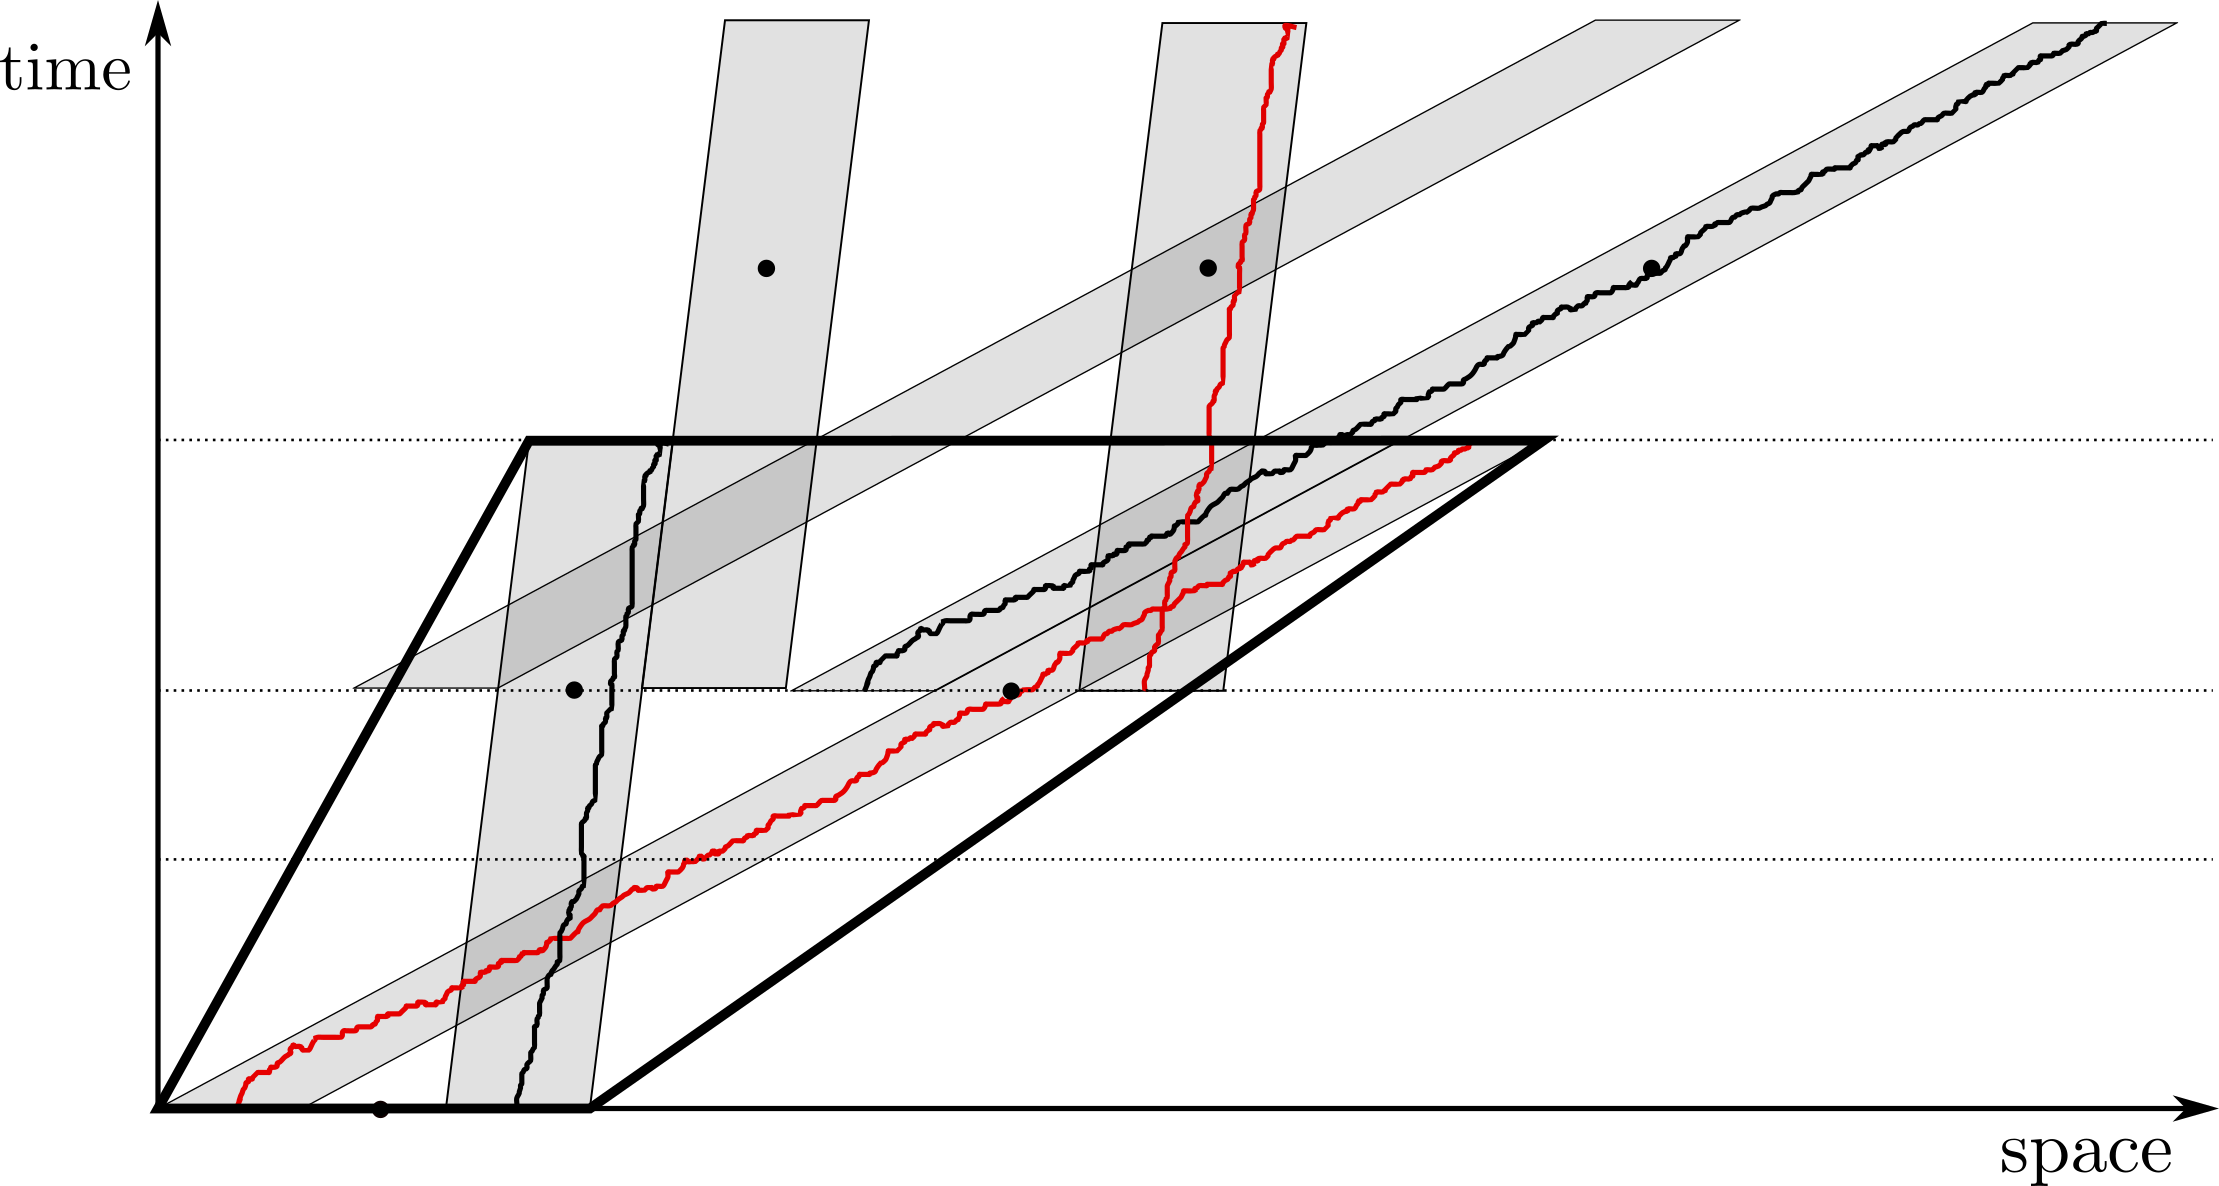
\includegraphics[scale=0.85]{images/simple_tiling}
\caption{Red path showing how oriented percolation to infinity occurs. }
\end{figure}
\end{frame}

\section{References}
\begin{frame}
\frametitle{References}
\printbibliography
%\bibliographystyle{alpha}
%\bibliography{bibliography_presentation}
\end{frame}
\end{document}